% Draft for arXiv / SQAI-NCTS Workshop 2027. Numbers come from results/*.json (see docs/qpinn_next_plan.md).
\documentclass[11pt]{article}
\usepackage[a4paper,margin=25mm]{geometry}
\usepackage{amsmath,amssymb,bm}
\usepackage{graphicx}
\usepackage{booktabs}
\usepackage{siunitx}
\usepackage[numbers,sort&compress]{natbib}
\usepackage{hyperref}
\graphicspath{{../figs/}}

\title{What does a quantum reservoir bring to physics-informed solid mechanics?\\
\large A fair benchmark against classical random features}
\author{[Author names] \\ [Affiliations]}
\date{Draft, \today}

\begin{document}
\maketitle

\begin{abstract}
Quantum physics-informed neural networks (QPINNs) are often reported with few parameters and
modest accuracy, but rarely against classical models of the same size that have been tuned with the same care.
We revisit the question for linear solid mechanics.
First, variational QPINNs lose to size-matched classical networks on Lam\'e, Kirsch and thermoelastic problems,
and the bottleneck is optimization rather than expressivity.
Second, we remove the optimization by freezing the circuit and solving only a linear readout by one least-squares solve
(a quantum extreme-learning or reservoir PINN, QERC-PINN).
With a per-qubit encoding and a Haar or Clifford+T reservoir, QERC-PINN reaches relative errors of
$\sim\!5\times10^{-5}$ on the Kirsch plate and resolves the stress concentration factor $K_t=3.00$.
Third, we show that the features $p_k(\bm x)=\mathrm{Tr}[U^\dagger|k\rangle\langle k|U\rho(\bm x)]$ are linear in the
encoded state, so the reservoir only selects a random $2^N$-dimensional subspace of the tensor-product function space
spanned by $\rho(\bm x)$; the encoding alone fixes what can be represented.
A classical random projection of the same tensor-product space reproduces the quantum results exactly.
On application problems with material interfaces --- a through-silicon via (TSV), periodic TSV arrays and
carbon-fibre unit cells --- the quantum reservoir matches a classical two-layer random network, while
cosine (Fourier) random features are best in almost every case, by up to $\sim\!40\times$.
Finally, measurement shot noise is the main obstacle on hardware: with $10^7$ shots per circuit the strong-form
solution still has errors of 4--11\%. Moving to an energy (Ritz) formulation that needs only first derivatives
reduces the error 3--4 times (about one order of magnitude in shots), but a further 2--3 orders of magnitude are needed.
We release all code and data.
\end{abstract}

% =====================================================================
\section{Introduction}
% TODO: motivation (PINNs for solid mechanics; QML claims of parameter efficiency); related work
% \citep{raissi2019pinn,dwivedi2020pielm,schuld2021encoding,ikeda2026qerc,qrfm2025,fspielm2026,hybridqpinn2026,qcpinn2025}.
Physics-informed neural networks (PINNs) \citep{raissi2019pinn} and their quantum counterparts (QPINNs)
\citep{qcpinn2025,hybridqpinn2026} are attractive for small-parameter surrogate models.
Claims of parameter efficiency, however, depend strongly on the classical baseline.
In this work we ask a narrower question with careful controls: \emph{for linear elasticity, what part of a quantum
model actually helps, and can a classical model with the same structure reproduce it?}

Our contributions are:
\begin{enumerate}
  \item A negative but diagnostic result for variational QPINNs: the bottleneck is optimization (Sec.~\ref{sec:vqpinn}).
  \item A QERC-PINN that avoids optimization by one least-squares solve, and a simple argument that the reservoir
        cannot change the representable function space (Sec.~\ref{sec:theory}).
  \item A fair benchmark with tuned classical random features, including cosine features and classical controls
        that share the tensor-product structure of the quantum features (Secs.~\ref{sec:kirsch}--\ref{sec:apps}).
  \item A shot-noise analysis and a first mitigation by an energy formulation (Sec.~\ref{sec:shots}).
\end{enumerate}

% =====================================================================
\section{Methods}
\subsection{Problems}
All problems are 2D linear elasticity in plane strain or plane stress:
$\nabla\cdot\bm\sigma=\bm 0$, $\bm\sigma=\lambda\,\mathrm{tr}\bm\varepsilon\,\bm I+2\mu\bm\varepsilon-\beta\Delta T\,\bm I$,
$\beta=(3\lambda+2\mu)\alpha$.
\begin{itemize}
  \item \textbf{Kirsch plate}: an infinite plate with a circular hole under uniaxial tension, truncated at $R$,
        with the exact displacement on the outer boundary and traction-free hole ($K_t=3$).
  \item \textbf{Single TSV}: a Cu via (radius $a$) in Si (outer radius $4a$), uniform cooling $\Delta T=-250$\,K.
  \item \textbf{Periodic TSV array}: square array with pitch $L$; a quarter cell with symmetric roller conditions
        (zero normal displacement and zero shear traction) under zero macroscopic strain.
  \item \textbf{CFRP fibre unit cell}: carbon fibre/epoxy square array with fibre volume fraction
        $V_f\in\{0.3,0.5,0.6\}$; longitudinal shear $G_{12}$ (a scalar Laplace problem) and transverse $C_{11}$
        (plane strain) under a unit macroscopic strain.
\end{itemize}
References are analytic (Kirsch, single TSV) or a P1 finite-element solution on an interface-fitted mesh with
$h=0.005a$, checked against $2h$ (differences $\le 3\times10^{-5}$ in displacement and $\le 10^{-5}$ in effective moduli).

\subsection{Least-squares PINN with fixed features}
The displacement in each material phase is $\bm u(\bm x)=\sum_k \bm c_k\phi_k(\bm x)$ with fixed features $\phi_k$.
PDE residuals at collocation points, boundary conditions and interface conditions
(continuity of $\bm u$ and of traction, with the thermal-mismatch jump) are all linear in $\bm c$, so the
coefficients follow from one regularized least-squares solve \citep{dwivedi2020pielm}.
Each phase has its own features.

\subsection{Features compared}
\begin{itemize}
  \item \textbf{QERC (quantum)}: per-qubit encoding $|\psi(\bm x)\rangle=\bigotimes_{l=1}^N
        \big(\cos\tfrac{\theta_l}{2}|0\rangle+e^{i\varphi_l}\sin\tfrac{\theta_l}{2}|1\rangle\big)$,
        with $2N$ angles from a random affine map of the input (as in \citet{ikeda2026qerc}),
        followed by a fixed reservoir $U$ (Haar, Clifford+T or transverse-field Ising evolution);
        the $2^N$ outcome probabilities $p_k(\bm x)=|\langle k|U|\psi(\bm x)\rangle|^2$ are the features.
  \item \textbf{tanh RF}: $\tanh(\bm w_k\cdot\bm x+b_k)$ \citep{rahimi2007rf}.
  \item \textbf{Fourier RF / Fourier PIELM}: $\cos(\bm w_k\cdot\bm x+b_k)$; FS-PIELM \citep{fspielm2026}.
  \item \textbf{Tensor random projection (classical control)}: $\mathrm{Re}\,\langle\psi(\bm x)|R_k|\psi(\bm x)\rangle$
        with the same $|\psi(\bm x)\rangle$ and independent GUE matrices $R_k$.
  \item \textbf{MLP2 (classical control)}: features of a random two-layer tanh network with $2N$ hidden units.
\end{itemize}
Every model has the same number of features ($2^N$) and its input scale is swept; for each seed we report the
best scale. This tuning was decisive: an untuned classical baseline looked equal to the quantum model with two
seeds, while the tuned one was $20\times$ better.

% =====================================================================
\section{Variational QPINNs are limited by optimization}\label{sec:vqpinn}
% TODO: table from 13_/19_ scripts (Lamé, Kirsch). Key numbers:
% Lamé: expressivity 7e-4 vs PDE training 5e-2 (72x). Kirsch: plain circuit saturates at 2e-1 (8 qubits);
% physics-aware encoding improves u by 2-3x but stays behind a 57-62 parameter MLP (8e-2).
On the 1D Lam\'e problem, a supervised fit of the analytic solution reaches $7\times10^{-4}$ while PDE training of
the same circuit stops at $5\times10^{-2}$. On the Kirsch plate, polar or Chebyshev encodings improve the
displacement error by 2--3 times, but a classical MLP of the same size with the same inputs stays ahead.
Since the analytic solution lies close to the circuit's function class, we attribute the gap to optimization.

% =====================================================================
\section{The reservoir does not change the function space}\label{sec:theory}
For any reservoir $U$, $p_k(\bm x)=\mathrm{Tr}[M_k\rho(\bm x)]$ with $M_k=U^\dagger|k\rangle\langle k|U$ and
$\rho(\bm x)=|\psi(\bm x)\rangle\langle\psi(\bm x)|$. Each feature is therefore a fixed linear combination of the
matrix elements of $\rho(\bm x)$, and
\begin{equation}
  \mathrm{span}\{p_k\}\subseteq\mathcal F_\rho=\mathrm{span}\{\rho_{ij}(\bm x)\}.
\end{equation}
With a linear readout, the reservoir can only pick a subspace of $\mathcal F_\rho$, which is fixed by the encoding.
Two consequences follow and are confirmed numerically (Fig.~\ref{fig:reservoir}):
(i) if every qubit receives the same input, $\dim\mathcal F_\rho$ is small and the reservoir does not matter
(changing the Ising time or couplings leaves the PDE error unchanged to three digits; at $N=8$ only 152 of 256
features are independent);
(ii) with a per-qubit encoding, $\dim\mathcal F_\rho$ grows like $4^N$ and a generic reservoir (Clifford+T, Ising, Haar)
improves the error by two orders of magnitude over no reservoir or a Clifford-only reservoir, in line with
\citet{ikeda2026qerc}.
The same argument shows that a classical random projection of $\mathcal F_\rho$ (tensor RP) has the same expressive
power as the quantum reservoir; the quantum device only provides access to $\mathcal F_\rho$ with $N$ qubits.

\begin{figure}[t]
  \centering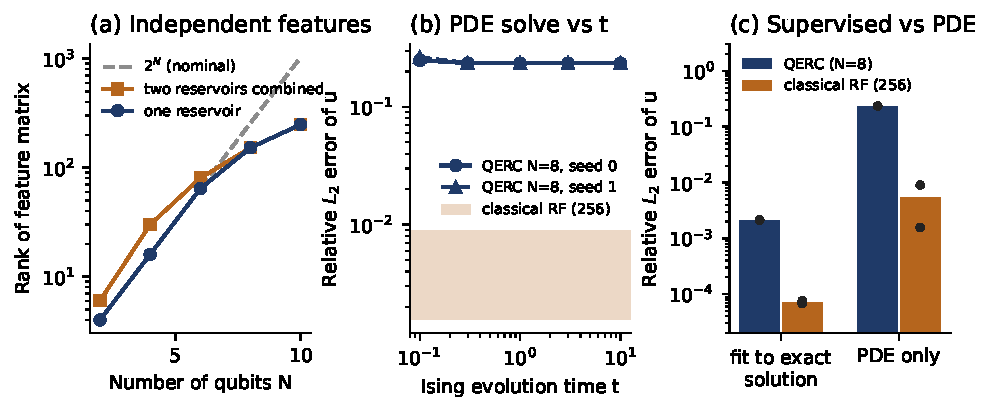
\includegraphics[width=\linewidth]{qerc_reservoir.pdf}
  \caption{Effect of the reservoir for per-qubit encoding (Kirsch, PDE only). TODO: update caption to the figure.}
  \label{fig:reservoir}
\end{figure}

% =====================================================================
\section{Fair comparison on the Kirsch plate}\label{sec:kirsch}
\begin{table}[t]
  \centering
  \caption{Kirsch plate, PDE only, $N=10$ (1024 features), 5 seeds, best input scale per seed.
           Relative $L_2$ error of displacement: geometric mean [min, max].}
  \label{tab:kirsch}
  \begin{tabular}{lc}
    \toprule
    Features & rel.\ $L_2(\bm u)$ \\
    \midrule
    QERC, Haar        & $4.6\times10^{-5}$ [$2.9\times10^{-5}$, $8.4\times10^{-5}$] \\
    QERC, Clifford+T  & $4.7\times10^{-5}$ [$2.4\times10^{-5}$, $9.7\times10^{-5}$] \\
    tanh RF           & $5.9\times10^{-5}$ [$3.2\times10^{-5}$, $1.0\times10^{-4}$] \\
    Fourier PIELM     & $\bm{1.1\times10^{-6}}$ [$4.8\times10^{-7}$, $1.9\times10^{-6}$] \\
    FS-PIELM          & $1.3\times10^{-6}$ [$4.4\times10^{-7}$, $6.2\times10^{-6}$] \\
    \bottomrule
  \end{tabular}
\end{table}
With tuned scales on both sides (Table~\ref{tab:kirsch}, Fig.~\ref{fig:fair}), the quantum reservoir and tanh
random features are equivalent, and both recover $K_t=3.00\pm0.03$.
Cosine features --- the classical analogue closest to the trigonometric quantum features --- are about $40\times$
more accurate.

\begin{figure}[t]
  \centering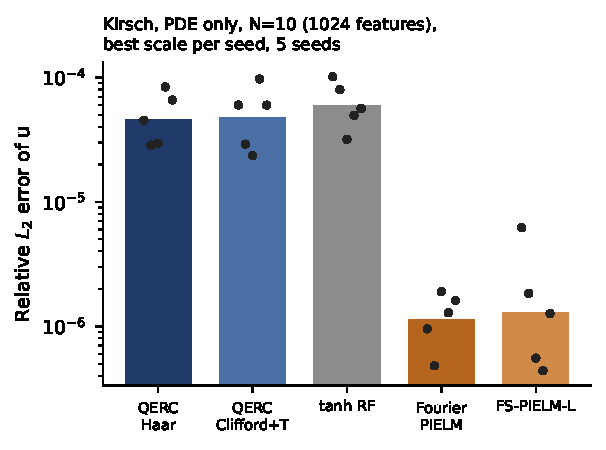
\includegraphics[width=0.8\linewidth]{qerc_fair_scales.pdf}
  \caption{Kirsch plate: all feature types with tuned input scale (5 seeds).}
  \label{fig:fair}
\end{figure}

% =====================================================================
\section{Problems with material interfaces}\label{sec:apps}
\subsection{Single TSV}
For a single Cu via in Si ($N=8$, 3 seeds), QERC reaches $3.9\times10^{-3}$, ten times better than one-layer tanh
($4.8\times10^{-2}$) or Fourier ($4.5\times10^{-2}$) features. The tensor random projection reproduces the
quantum result exactly ($3.84\times10^{-3}$ vs $3.85\times10^{-3}$, with matching per-seed and per-scale trends;
Fig.~\ref{fig:tsvctrl}), and a random two-layer network reaches $1.4\times10^{-2}$.
The advantage over one-layer features therefore comes from the product structure of $\mathcal F_\rho$, not from
anything specific to quantum measurement.

\begin{figure}[t]
  \centering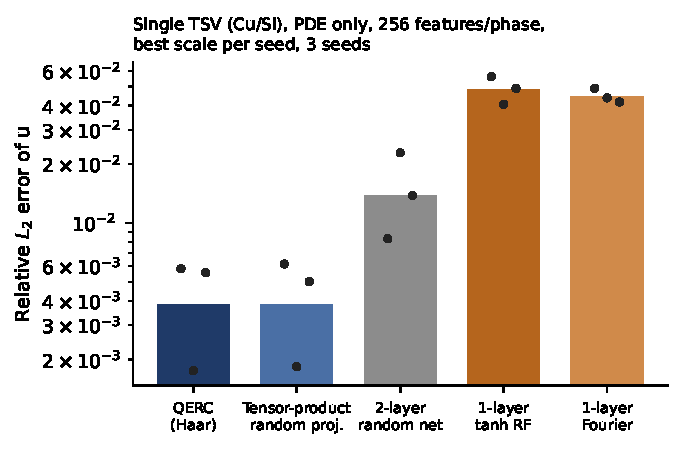
\includegraphics[width=0.8\linewidth]{tsv_controls.pdf}
  \caption{Single TSV: quantum reservoir and classical controls.}
  \label{fig:tsvctrl}
\end{figure}

\subsection{Periodic TSV array}
For the quarter unit cell (Fig.~\ref{fig:tsvpitch}), cosine features are best for narrow pitches
($L=3,4$: $1.4\times10^{-5}$ and $2.7\times10^{-5}$, close to the FE reference accuracy).
For wider pitches the cosine features degrade fastest ($L=10$: $4.4\times10^{-3}$ vs $1.0\times10^{-3}$ for QERC).
This is not a collocation-density effect (doubling the points changes nothing) but a feature-count effect:
with 1024 features at $L=6$, all models drop to $\sim\!10^{-5}$ and the cosine features are again best
($5.9\times10^{-6}$). Across all pitches, QERC and MLP2 agree within the seed spread.

\begin{figure}[t]
  \centering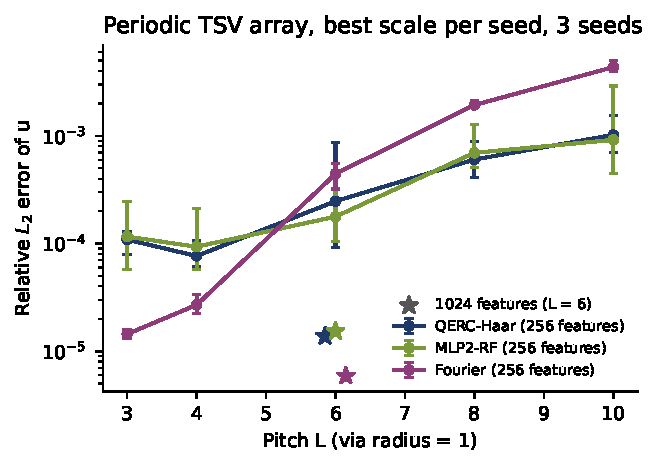
\includegraphics[width=0.6\linewidth]{tsv_pitch.pdf}
  \caption{Periodic TSV array: displacement error versus pitch $L$ (256 features; stars: 1024 features at $L=6$).}
  \label{fig:tsvpitch}
\end{figure}

\subsection{CFRP fibre unit cell}
All models predict the effective moduli to better than $10^{-3}$ (Fig.~\ref{fig:cfrp}).
Cosine features are best in all cases, by about $20\times$ for $C_{11}$ at $V_f\ge0.5$
(e.g.\ $8.4\times10^{-6}$ vs $1.6\times10^{-4}$ for QERC at $V_f=0.5$).
QERC again matches MLP2. As a check of the reference, the FE value of $G_{12}$ agrees with Halpin--Tsai
($\xi=1$) \citep{affdl1976halpintsai} to 0.1\% at $V_f=0.3$ and deviates by 4\% at $V_f=0.6$, as expected for a
square array.

\begin{figure}[t]
  \centering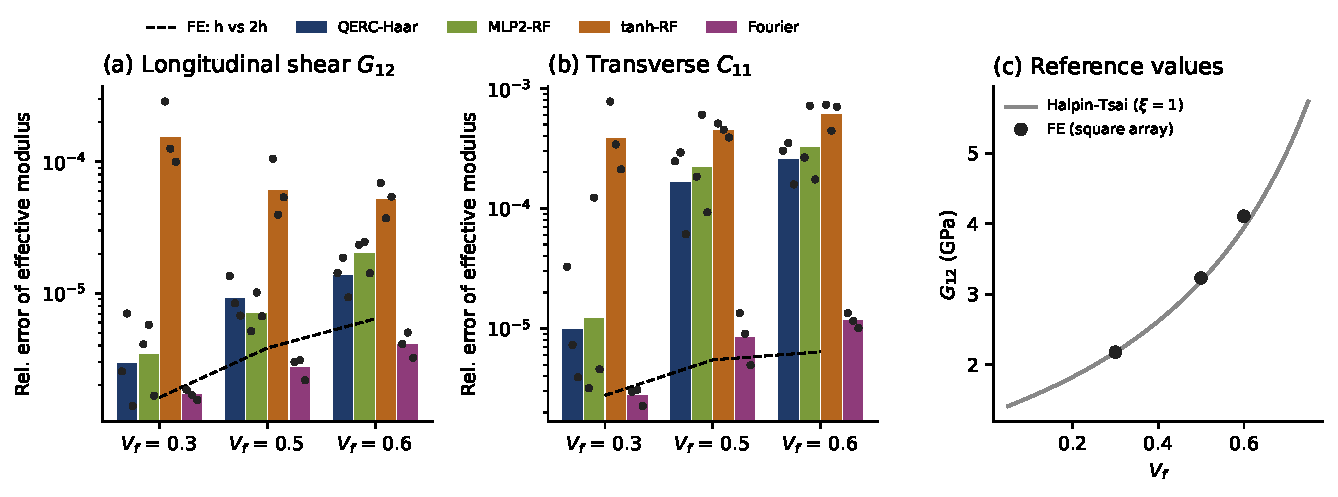
\includegraphics[width=\linewidth]{cfrp_unitcell.pdf}
  \caption{CFRP unit cell: relative error of the effective moduli $G_{12}$ and $C_{11}$ (3 seeds), and the FE reference.}
  \label{fig:cfrp}
\end{figure}

\subsection{A high-dimensional counterexample}
One may expect the exponential tensor-product space to help when the input is high-dimensional.
For the dispersion relation of a $d$-layer laminate ($d=N$ inputs), whose exact solution lies in the $2^N$-dimensional
span of $\bigotimes_i(\cos\varphi_i,\sin\varphi_i)$, all random feature models fail (relative error $>1$), quantum
or classical: a random reservoir picks a random $2^N$-dimensional subspace of a $3^N$--$4^N$-dimensional space, whose
overlap with the target shrinks exponentially. A benefit would require a reservoir designed for the problem.

% =====================================================================
\section{Shot noise and an energy formulation}\label{sec:shots}
On hardware, $p_k$ and its derivatives are estimated from $S$ shots per circuit, with derivatives from the
parameter-shift rule \citep{mitarai2018qcl,schuld2019gradients}.
We propagate the multinomial variance $p(1-p)/S$ through the chain rule (an approximate model that ignores
correlations between circuits) and add the noise only when assembling the system.
Since $p_k\approx 2^{-N}$, the relative noise per feature scales as $\sqrt{2^N/S}$, and second derivatives amplify it.

\begin{table}[t]
  \centering
  \caption{Kirsch, $N=10$, Haar reservoir, 2 seeds: relative $L_2(\bm u)$ versus shots per circuit.
           Ridge and boundary penalty chosen by the test error for all methods (optimistic bound).}
  \label{tab:shots}
  \begin{tabular}{lcccc}
    \toprule
    Shots & Strong form & Strong, split shots & Energy (Ritz) & Energy, split shots \\
    \midrule
    $10^3$ & 0.46 & 0.72 & \textbf{0.32} & 0.66 \\
    $10^5$ & 0.25 & 0.25 & \textbf{0.083} & 0.16 \\
    $10^7$ & 0.062 & 0.13 & \textbf{0.014} & 0.035 \\
    $\infty$ & $6.3\times10^{-4}$ & -- & $\bm{2.1\times10^{-4}}$ & -- \\
    \bottomrule
  \end{tabular}
\end{table}

The energy (Ritz) formulation \citep{nguyen2020dem} minimizes
$\tfrac12\int\bm\varepsilon:\mathbb C:\bm\varepsilon\,dA$ plus a boundary penalty, so the stiffness matrix needs
only first derivatives; the traction-free hole is a natural boundary condition.
It reduces the error 3--4 times at every shot level and recovers $K_t=3.0$ from $10^5$ shots, where the strong form
gives 1.4 (Table~\ref{tab:shots}, Fig.~\ref{fig:shots}).
Splitting the shots into two independent halves removes the noise-squared bias of the normal matrix but makes the
results worse: the bias acts as a ridge regularizer. Fewer qubits reduce the relative noise but lose
expressivity ($N=6$ saturates at 0.2).
Even so, $10^7$ shots per circuit still give 1.4\% error, 70 times the noiseless value.

\begin{figure}[t]
  \centering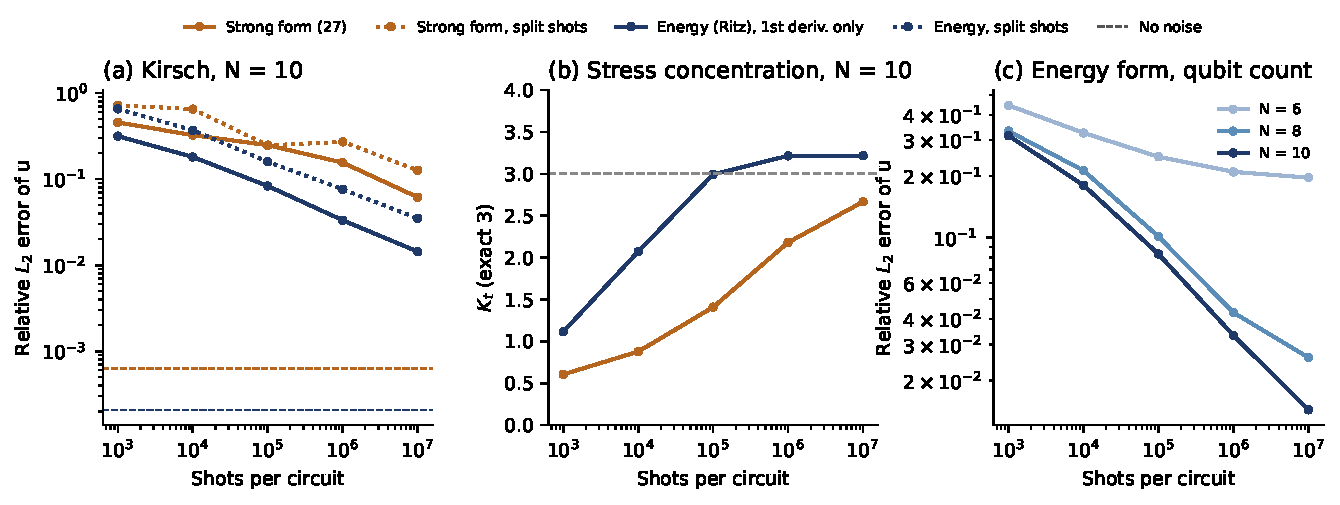
\includegraphics[width=\linewidth]{shot_mitigation.pdf}
  \caption{Shot noise: strong versus energy formulation, with and without split-shot estimation, and qubit count.}
  \label{fig:shots}
\end{figure}

% =====================================================================
\section{Discussion}
% TODO: expand.
\begin{itemize}
  \item The design freedom of a quantum reservoir PINN lies in the encoding. The reservoir only needs to be generic.
  \item Whatever advantage appears over simple classical features is reproduced by a classical model with the same
        tensor-product structure; the quantum claim reduces to accessing $\mathcal F_\rho$ with $N$ qubits,
        which matters only when $4^N$ classical cost is prohibitive.
  \item Tuning of the classical baseline changes conclusions by more than an order of magnitude and must be reported.
  \item Shot noise, not expressivity, limits hardware use. Formulations with low derivative order and readouts with
        larger probabilities (few observables instead of $2^N$ outcomes) are the next steps.
\end{itemize}

\section{Conclusion}
% TODO
For linear solid mechanics, a quantum reservoir with least-squares readout is a working PINN solver, but under a fair
comparison it matches classical random features with the same structure and trails cosine features.
We hope the benchmark and the controls serve as a baseline for future claims.

\paragraph{Code and data.} \url{https://github.com/mmc-research-group/nishioka-qpinn-solid}

\bibliographystyle{unsrtnat}
\bibliography{refs}
\end{document}
